% Created 2022-01-26 Wed 22:01
% Intended LaTeX compiler: xelatex
\documentclass[11pt,twoside,landscape]{article}
\usepackage{graphicx}
\usepackage{longtable}
\usepackage{wrapfig}
\usepackage{rotating}
\usepackage[normalem]{ulem}
\usepackage{amsmath}
\usepackage{amssymb}
\usepackage{capt-of}
\usepackage{hyperref}
\usepackage[newfloat]{minted}
\usepackage{color}
\usepackage{listings}
\usepackage[top=2cm,bottom=2cm,right=2cm,left=2cm,landscape]{geometry}
\usepackage{multicol}
\usepackage{enumitem}
\usepackage{fancyhdr}
\setlist{noitemsep}
\setlength{\parindent}{0pt}
\setlength{\columnseprule}{0.2pt}
\definecolor{mygreen}{rgb}{0,0.6,0}
\definecolor{mygray}{rgb}{0.5,0.5,0.5}
\definecolor{mymauve}{rgb}{0.58,0,0.82}
\lstset{ backgroundcolor=\color{white}, basicstyle=\footnotesize, breaklines=true, captionpos=b, commentstyle=\color{mygreen}, escapeinside={\%*}{*)},keywordstyle=\color{blue}, stringstyle=\color{mymauve},}
\author{Olivier Lischer}
\date{\today}
\title{MsTe Summary}
\hypersetup{
 pdfauthor={Olivier Lischer},
 pdftitle={MsTe Summary},
 pdfkeywords={},
 pdfsubject={},
 pdfcreator={Emacs 27.2 (Org mode 9.5.2)}, 
 pdflang={English}}
\begin{document}

\pagestyle{fancy}
\fancyhf{}
\fancyhead[R]{MsTe-HS21}
\fancyhead[L]{Exam Summary}
\fancyfoot[CE,CO]{\leftmark}
\fancyfoot[R]{\thepage}
\fancyfoot[L]{Olivier Lischer}
\begin{multicols}{3}

\section{.NET}
\label{sec:orgf8f6835}
\textbf{.NET}

\begin{itemize}
\item .NET Framework: only for Windows, no new Updates (except security patches)
\item .NET Core: new runtime, crossplatform
\item .NET: successor of .NET Core. This should be used today
\end{itemize}

\begin{center}
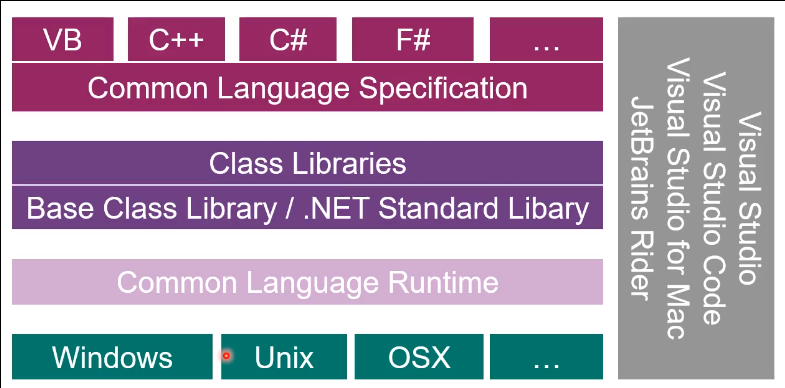
\includegraphics[width=.9\linewidth]{img/dot_net_architektur.png}
\label{org3754dcb}
\end{center}

\textbf{.NET Standard}

The .NET Stadard is used to establish a compatibility between different implementation.
The standard defines which functions, classes, etc. a implementation has to provided to be conform. 

\textbf{Common Language Runtime (CLR)}

The Common Language Runtime (CLR) has:
\begin{itemize}
\item a JIT Compiler which compiles the \href{../../../roam/20211003114528-microsoft_intermediate_language.org}{Microsoft Intermediate Language} to native code
\item Garbage Collection
\item inter language debugging
\item thread management
\end{itemize}


\begin{center}
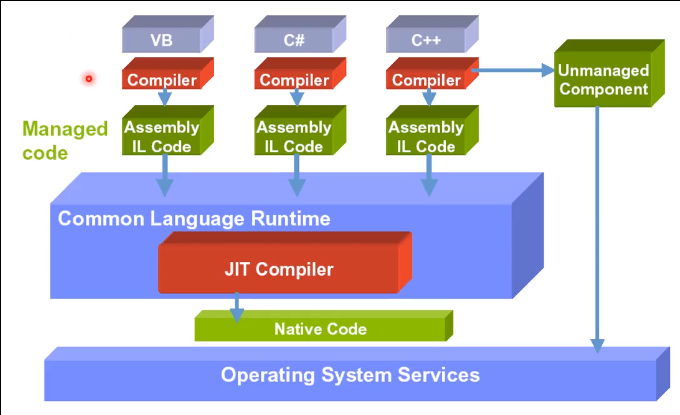
\includegraphics[width=.9\linewidth]{img/clr_architektur.png}
\label{org97ec0a6}
\end{center}

\textbf{Common Type System}

Common Type System (CTS) is the standard in \href{../../../roam/20211003114703-net.org}{.NET} how a type definitions and specific values are stored in memory.
All types in .NET inherit from \texttt{System.Object}. Also types like int, long and float inherit from \texttt{System.Object}. In CTS exists two different kind of types: Reference types (\texttt{class} keyword) and Value types (\texttt{struct} keyword). Value types are stored on the stack and are automatically boxed if it is used with something like a list, which stores its  element on the heap. 

\begin{table}[htbp]
\label{tab:org2a2b91b}
\centering
\begin{tabular}{lll}
 & Reference (Class) & Value (Struct)\\
\hline
Memory Location & heap & stack\\
Variable contains & reference & value\\
Null value & possible & never\\
Default value & null & 0, false, '$\backslash$0'\\
Assignment / Call & copy reference & copy value\\
derivation possible & yes & no (sealed)\\
\end{tabular}
\end{table}

Each type has always a reference to the type description 

\begin{center}
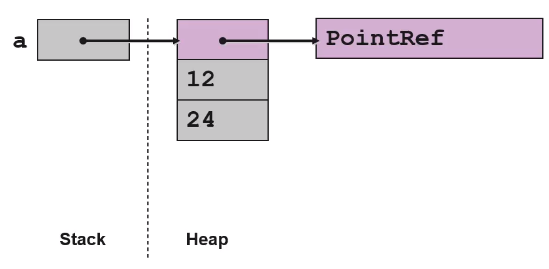
\includegraphics[width=.9\linewidth]{img/ref_type_stack_heap.png}
\label{org6141b25}
\end{center}

\textbf{.NET Assembly}

After the compilation you receive an Assembly.
This could be an *.exe or *.dll in Windows.
This Assembly is dynamically loadable and contains meta data.
It something like the JAR file in \href{../../../roam/20201116150053-java.org}{Java}.

\textbf{What contains a .NET Assembly?}

The Assembly contains:
\begin{itemize}
\item Manifest (references to other assemblies, metadata, version, author, \ldots{})
\item Module (types)
\item Resources  (images, translations files, \ldots{})
\end{itemize}


Module metadata:
\begin{itemize}
\item public, private, \ldots{}
\item describes all aspect of the code except programming logic
\item used to guarantee type safety
\item is normally used in IDEs to provide auto complition
\end{itemize}


\textbf{Microsoft Intermediate Language (MSIL)}

MSIL is similar to assembler but is platform independent.
The MSIL is the same for all \href{../../../roam/20211003114703-net.org}{.NET} languages.
The benefits of the MSIL are:
\begin{itemize}
\item portability
\item typesafety
\end{itemize}

The drawback is that the normal compiled project is not as efficient as native code.
But you can compile a \href{../../../roam/20211003114703-net.org}{.NET} project direct in native code.

\textbf{MSIL in Action}

\begin{itemize}
\item Design Time (platform independent, development, MSIL)
\item Run Time (platform dependent, JIT)
\end{itemize}

JIT Compilation:
compiled method calls an IL function.
The runtime detects that this function is not compiled yet and calls the JIT compiler.
The JIT compiler translate the IL code in native code and replace the IL code with native code in the memory.

\textbf{.NET reference types}

In \href{../../../roam/20211003114703-net.org}{.NET} exists 4 different kinds of references:
\begin{itemize}
\item precompiled assemblies (not possible to debug), \texttt{<Reference> ... </Reference>}
\item \href{../../../roam/20211003140935-nuget_package.org}{NuGet Package} (external dependency, not possible to debug), \texttt{<PackageReference> ... </PackageReference>}
\item Visual Studio Project (in same solution), \texttt{<ProjectReference> ... </ProjectReference>}
\item SDK (required, default classes)
\end{itemize}


\textbf{C\# Project Files}

The \href{../../../roam/20211003114703-net.org}{.NET} project are store in a XML file.
In a \href{../../../roam/20211003114158-c.org}{C\#} project the file is called *.csproj.
The most important part in the file are:
\begin{itemize}
\item PropertyGroup: Settings
\item ItemGroup: item which should be compiled
\item TargetGroup: a sequence of step to execute
\end{itemize}

\section{C\#}
\label{sec:org7d2d6e0}

\begin{center}
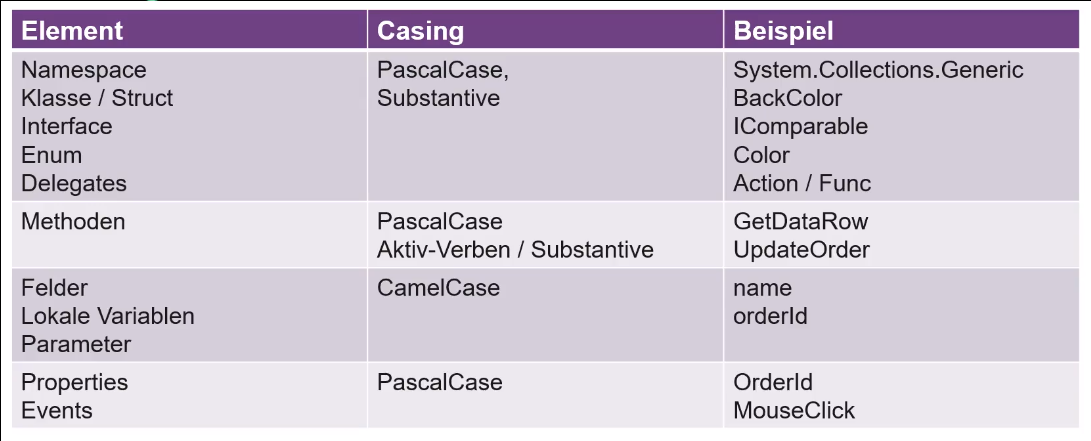
\includegraphics[width=.9\linewidth]{img/naming_guidelines.png}
\label{org69da6ad}
\end{center}

\begin{center}
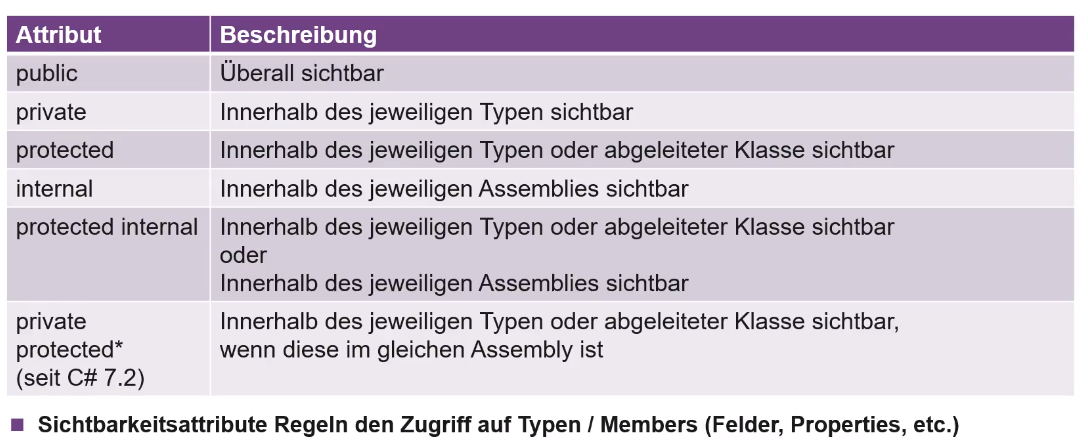
\includegraphics[width=.9\linewidth]{img/sichtbarkeitsattribute.png}
\label{org9f4e36c}
\end{center}


\textbf{Namespaces in C\#}

Namespaces are similar to the packages in \href{../../../roam/20201116150053-java.org}{Java}.
But in \href{../../../roam/20211003114158-c.org}{C\#} the file systems does not have correspond the the namespace.
But it is best practice to have the same hierarchy.
A namespace can be renamed during the import: \texttt{using F = System.Windows.Forms}

\textbf{Main Method in C\#}

The main method in \href{../../../roam/20211003114158-c.org}{C\#} can exits mulitple times.
If this is the case the corret starting method has to written in the *.csproj file:

\lstset{language=XML,label= ,caption= ,captionpos=b,numbers=none}
\begin{lstlisting}
<StartupObject>CSharpGrundlagen_Main01.Program1</StartupObject>
\end{lstlisting}

\begin{center}
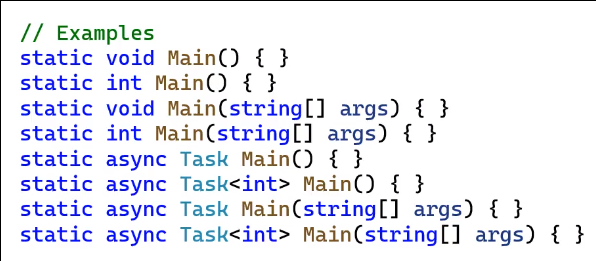
\includegraphics[width=.9\linewidth]{img/main_methods_example.png}
\label{orgb9b1b9f}
\end{center}

Arguments can be access with:
\lstset{language=csharp,label= ,caption= ,captionpos=b,numbers=none}
\begin{lstlisting}
string[] args;
System.Environment.GetCommandLineArgs();
System.CommandLine; /*NuGet*/
\end{lstlisting}


The main method is not required.
If you leave out the main method (only allowed once) the following schema is required:
\begin{itemize}
\item usings
\item the code which is normaly in main
\item functions / enums / classes / structs \ldots{}
\end{itemize}


The argument array is then always called args.

\lstset{language=csharp,label= ,caption= ,captionpos=b,numbers=none}
\begin{lstlisting}
using System;

Volume vLow = Volume.Low;
PrintVolume(vLow);

static void PrintVolume(Volume volume) { /* */ }
public enum Volume { /* */ }
\end{lstlisting}

\textbf{Enums in C\#}

Enums in \href{../../../roam/20211003114158-c.org}{C\#} are only a list with predefined constants (default Int32).
Normally the first value is a 0 and the incremented.
It is possible to define the int value explicitly (\texttt{enum Days \{Sunday = 10, ... \}}.
After that the value is incremented again.
It is possible that the enum has for different options the same int value.
This could happens when you set one option explicit higher and one option explicit lower.
In this case it is not recommended to convert the int in an enum (it will always take only the first option).

To save memory you can adjust the used type \texttt{enum Days : byte \{ Sunday, Monday ... \};}.
This is \emph{not in inheritance}. Just a hint for the compiler.

\textbf{String to Enum}

Often you want to convert a String into an Enum (\href{../../../roam/20211006113326-enums_in_c.org}{Enums in C\#}).
For this operation you have to options:
\begin{itemize}
\item The Option 1 should not be used anymore, because it can throw exceptions
\item Option 2 and 3 are identical except that Option 3 has same syntactical sugar.
\end{itemize}

\lstset{language=csharp,label= ,caption= ,captionpos=b,numbers=none}
\begin{lstlisting}
// Option 1
Days day1 = (Days)Enum.Parse(typeof(Days), "Monday");

// Option 2
Days day2;
bool success2 = Enum.TryParse("Monday", out day2);

// Option 3
bool success3 = Enum.TryParse("Monday", out Days day3); // C# 7.0
\end{lstlisting}

\textbf{Print all Options of an Enum}

Sometimes you want to iterate over all Values of a enum (\href{../../../roam/20211006113326-enums_in_c.org}{Enums in C\#}).

\lstset{language=csharp,label= ,caption= ,captionpos=b,numbers=none}
\begin{lstlisting}
foreach (string day in Enum.GetNames(typeof(Days)))
{
    Console.WriteLine(day);
}
\end{lstlisting}

\textbf{String in C\#}

The type string is a reference type (class) but behaves like a Value type and are reused internally.
Only \texttt{string.Copy()} creates a real new copy.
Strings are immutable and value comparison with \texttt{=} / \texttt{!=} and \texttt{Equals} are possible (not like in \href{../../../roam/20201116150053-java.org}{Java}).
For escaping two methods exist:
\begin{itemize}
\item escaping with a backslash ($\backslash$): \texttt{"C:\textbackslash{}\textbackslash{}"}
\item or with a at @: \texttt{@"C:\textbackslash{}"}
\end{itemize}


Strings should not be created with \texttt{string.Format()} or with the \texttt{+} operator.
The better way is string interpolation: \texttt{string s3 = \$"\{DateTime.Now\}: \{"Hello"\}";}

\textbf{Arrays in C\#}

In \href{../../../roam/20211003114158-c.org}{C\#} the array is a reference type is therefore stored on the heap.
It exists three different kind of arrays:
\begin{itemize}
\item \href{../../../roam/20211008083138-single_dimensional_arrays_in_c.org}{Single Dimensional Arrays in C\#}
\item \href{../../../roam/20211008083241-multidimension_array_in_c.org}{Multidimension Array in C\#}
\item \href{../../../roam/20211008083300-jagged_arrays_in_c.org}{Jagged Arrays in C\#}
\end{itemize}


If the array stores reference types then only the reference is stored in the array. If the array should store value types then these elements are automatically boxed (moved to the heap) and stored as a whole in the array.

\begin{center}
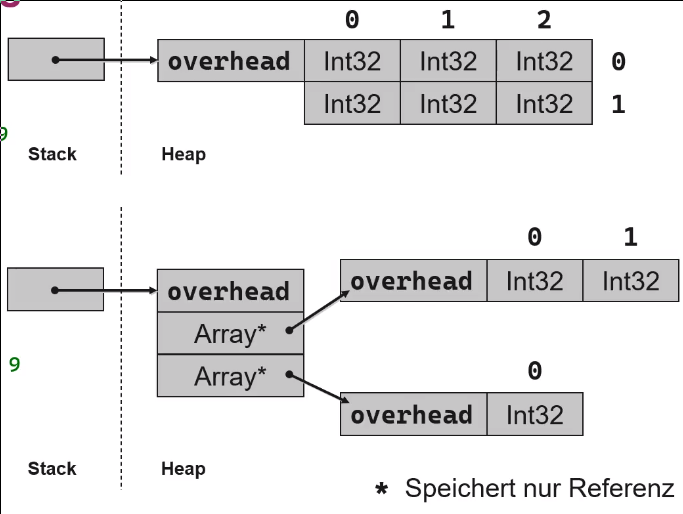
\includegraphics[width=.9\linewidth]{img/array_memory_layout.png}
\label{org0bfe442}
\end{center}

\textbf{Single Dimensional Array}

An plan old array. Nothing special.
\lstset{language=csharp,label= ,caption= ,captionpos=b,numbers=none}
\begin{lstlisting}
int[] array1 = new int[5];
int[] array2 = new int[] { 1, 4, 6};
int[] array3 = int[] {1,5,7};
int[] array4 = {1,3,5,5};
object[] array5 = new object[5];
\end{lstlisting}

\textbf{Multidimensional Array}

Multidimensional Arrays are also called Block Matrices because they look like a rectangle.

\lstset{language=csharp,label= ,caption= ,captionpos=b,numbers=none}
\begin{lstlisting}
int[,] multiDim1 = new int[2,3];
int[,] multiDim2 = new { {1,2,3}, {4,5,6}};

int[,] array = new int[3,2];
int length = array.Length; // 6
int length0 = array.GetLength(0); // 3
int length1 = array.GetLength(1); // 2
\end{lstlisting}


The benefits over \href{../../../roam/20211008083300-jagged_arrays_in_c.org}{Jagged Arrays in C\#} they are:
\begin{itemize}
\item more memory efficient
\item faster allocation
\item faster \href{../../../roam/20211008083744-garbage_collection.org}{Garbage Collection}
\end{itemize}


But the access to the elements are slower than in a \href{../../../roam/20211008083300-jagged_arrays_in_c.org}{Jagged Arrays in C\#}.
This is because the Boundary Check is in a \href{../../../roam/20211008083138-single_dimensional_arrays_in_c.org}{One Dimensional Array} is optimized.
This does not apply for Block Matrices. 

\textbf{Jagged Arrays}

Jagged Arrays are Arrays of Arrays.
From the first array, each index points to an indepentend Array.
They are called jagged (de: zerklüftet) because each array from the second array can have diffrent sizes.

\lstset{language=csharp,label= ,caption= ,captionpos=b,numbers=none}
\begin{lstlisting}
int[][] jaggedArray = new int[6][];
jaggedArray[0] = new int[] {1,2,3,4};

int[][] array1 new int[2][];
array1[0] = new int[3];
array1[1] = new int[1];
int length = array1.Length; // 2
int length0 = array1[0].Length; // 3
int length1 = array1[1].Length // 1
\end{lstlisting}

The access to the elements is in Jagged Arrays faster than in \href{../../../roam/20211008083241-multidimension_array_in_c.org}{Block Matrices} because the Boundary Check is for \href{../../../roam/20211008083138-single_dimensional_arrays_in_c.org}{One Dimensional Array} optimized.

\textbf{Structs in C\#}

In \href{../../../roam/20211003114158-c.org}{C\#} \texttt{struct} are value types and therefore live on the stack.
Derivation of a struct is not possible but a struct can implement interfaces.
Different as by classes you can not initialize the values directly:
\lstset{language=csharp,label= ,caption= ,captionpos=b,numbers=none}
\begin{lstlisting}
struct Point {
    int x = 0; // Compilerrror
    int y;

    Point(int x, int y) {
	this.x = x;
	this.y = y;
    }
}

\end{lstlisting}


Structs should only used in the following cases:
\begin{itemize}
\item to group primitives as one data type (like a Point)
\item the new type should be immutable
\item is not often boxed
\item short life span
\item or is embedded in other objects
\end{itemize}


\textbf{readonly fields}

In \href{../../../roam/20211003114158-c.org}{C\#} besides \texttt{const} there is also a \texttt{readonly}.
The value for a \texttt{readonly} fields does not have to be known at compile time.
The value can be calculated during deklaration or inside the constructor.

\textbf{nested types in}

The outer class has access to the public functions / fields / properties of the class.
But the inner class has access to everything of the outer class.
Foreign classes can access only on public functions / fields / properties and only if the class itself is public.

\textbf{Static Usings}

In \href{../../../roam/20211003114158-c.org}{C\#} you can import static classes / enums with static usings:
\lstset{language=csharp,label= ,caption= ,captionpos=b,numbers=none}
\begin{lstlisting}
using static System.Console;

WriteLine("Hello World");
\end{lstlisting}

If a naming clash occurs the normal overloading rules apply.
With the class name you can ensure the correct function call.

\textbf{Params}

In \href{../../../roam/20211003114158-c.org}{C\#} exists two kind of functions calls:
\begin{itemize}
\item call by value
\item call by reference
\end{itemize}


For call by reference exists two keywords with different purpose:
\begin{itemize}
\item \texttt{ref} (normal call be reference)
\item \texttt{out}
\end{itemize}


For overloading \texttt{ref} / \texttt{out} are distinguished feature.

\textbf{out Parameters}

A function which takes \texttt{out} parameters initialized this arguments during the function call.
This technique is used by the \texttt{TryParse} methods.
If you are not interested in one of the parameters then use the \texttt{\_} to discard the "return value".

\lstset{language=csharp,label= ,caption= ,captionpos=b,numbers=none}
\begin{lstlisting}
void Init(out int a, out int b) { a = 1; b = 2; }
void TestInit() { Init(out int a1, out _); }
\end{lstlisting}

\textbf{params array}

The params array allows the caller to add any number of arguments at the end:
\lstset{language=csharp,label= ,caption= ,captionpos=b,numbers=none}
\begin{lstlisting}
void DoSomething(string str, params string[] list) { /**/ }
DoSomething("{0} some string {1}", 2, 3); 
\end{lstlisting}

It has to be the last parameter in the function. During compilation time the parameters are transformed in an normal array. It is not possible to use the parms array with the \texttt{out} / \texttt{ref} keyword.

\textbf{Imporent}: the following two functions are the same for the compiler (no valid overloading):
\lstset{language=csharp,label= ,caption= ,captionpos=b,numbers=none}
\begin{lstlisting}
void DoSomething(string str, params string[] list) { /**/ }
void DoSomething(string str, string[] list) { /**/ }
\end{lstlisting}

\textbf{Optional Parameters}

In \href{../../../roam/20211003114158-c.org}{C\#} exist optional parameters.
This is realized that some parameters have a default value:
\lstset{language=csharp,label= ,caption= ,captionpos=b,numbers=none}
\begin{lstlisting}
void optionalParameters(int i, bool flag = true) { /**/ }
\end{lstlisting}

The default value has be calculated during compile time.
Leaving out an optional parameter is only possible at the end.
If you want to specify the last option then you have set all previous flags too.

\textbf{Important}: Default parameters are no distinguished feature for overloading.
The following are the same function for the compiler (compiler error):
\lstset{language=csharp,label= ,caption= ,captionpos=b,numbers=none}
\begin{lstlisting}
void optionalParameters(int i, bool flag = true) { /**/ }
void optionalParameters(int i, bool flag) { /**/ }
\end{lstlisting}

\textbf{Named Parameters}

The problem with \href{../../../roam/20211008100451-optional_parameters_in_c.org}{Optional Parameters in C\#} is that you have sometimes to specify every option even if you want only to change the default value of the last argument.
With named parameters this problem does not occur:
\lstset{language=csharp,label= ,caption= ,captionpos=b,numbers=none}
\begin{lstlisting}
void PrintOrderDetails(string productName, string sellerName, int orderNum) { /**/ }
PrintOrderDetails(orderNum: 31, productName: "Red Mug", sellerName: "Gift Shop");
\end{lstlisting}

\textbf{Properties}

Properties are compiler feature which implements the Getter and Setter methods.
In the Set part you can access the assigned value using the \texttt{value} keyword.

\lstset{language=csharp,label= ,caption= ,captionpos=b,numbers=none}
\begin{lstlisting}
public int LengthAuto { get; set; }
\end{lstlisting}

Auto implemented properties use compiler also a compiler feature.
To avoid naming conflicts the compiler creates a "unspeakable variable name".
This is a variable name which the compiler not accepted from the user.

You can even initialized auto implemented properties.
The set part does not even to be there.
\lstset{language=csharp,label= ,caption= ,captionpos=b,numbers=none}
\begin{lstlisting}
public string FirstName { get; set; } = "Jane"; 
\end{lstlisting}


Another compiler feature is that you can set the values over the Setters right after the creation using the default compiler:
\lstset{language=csharp,label= ,caption= ,captionpos=b,numbers=none}
\begin{lstlisting}
MyClass mc = new MyClass()
{
    Length = 1,
    Width = 2
};

// compiles to this
MyClass mc = new MyClass();
mc.Length = 1;
mc.Width = 2;
\end{lstlisting}

\textbf{Indexers}

Indexer are just a special case of \href{../../../roam/20211008103108-properties_in_c.org}{Properties in C\#}.
It is basically an overloading of the index operator (\texttt{[]}):
\lstset{language=csharp,label= ,caption= ,captionpos=b,numbers=none}
\begin{lstlisting}
MyClass mc = new MyClass();
mc[0] = "Hello";
string value1 = mc[0];

class MyClass
{
    private string[] arr = new string[10];
    // this zeigt an dass es ein indexer ist
    public string this[int index]
    {
	get { return arr[index]; }
	set { arr[index] = value; // value ist ein string in diesem fall }
    }

}
\end{lstlisting}

\textbf{Switch Expressions}

The switch expression in \href{../../../roam/20211003114158-c.org}{C\#} works like the switch expression in \href{../../../roam/20200904153952-rust.org}{Rust}.

\lstset{language=csharp,label= ,caption= ,captionpos=b,numbers=none}
\begin{lstlisting}
public static Orientation ToOrientation(Direction direction) => direction switch
{
    Direction.Up    => Orientation.North,
    Direction.Right => Orientation.East,
    Direction.Down  => Orientation.South,
    Direction.Left  => Orientation.West,
    _ => throw new ArgumentOutOfRangeException(nameof(direction), $"Not expected direction value: {direction}"),
};
\end{lstlisting}

\textbf{Default in C\#}

In \href{../../../roam/20211003114158-c.org}{C\#} for a \href{../../../roam/20211008085202-struct_in_c.org}{Struct in C\#} the default constructor is always available.
For a class when no constructor is implemented by the user or explicitly implemented.
In a \href{../../../roam/20211008085202-struct_in_c.org}{Struct in C\#} always all fields have to be initialized.

Using \texttt{default(T)} or \texttt{default} the memory location is filled with 0.
So the get the default value back.

\textbf{Static Constructors}

A static constructor is for structs and classes identically and has never parameters and no visibility.
The static constrocutr is used for initial work and is executed exactly once for the whole application during the first creation of an object of the class / struct.

\textbf{Operator Overloading}

The function has to be a \texttt{static} and needs the keyword \texttt{operator} with the operator afterwards:
\lstset{language=csharp,label= ,caption= ,captionpos=b,numbers=none}
\begin{lstlisting}
public static Point operator+(Point lhs, Point rhs) {
    return new Point(rhs.X + lhs.X, rhs.Y + lhs.Y);
}
\end{lstlisting}

The return type freely selectable.
But min. one parameter has to be from the same type of the class.

\textbf{Partial Class}

A class can be spitted in multiple files.
This requires the keyword \texttt{partial}.
This works with classes, structs and interfaces.
\lstset{language=csharp,label= ,caption= ,captionpos=b,numbers=none}
\begin{lstlisting}
// File1.cs
partial class MyClass
{
    public void Test1() {}
}

// File2.cs
partial class MyClass
{
    public void Test2() {}
}
\end{lstlisting}

Usage:
\begin{itemize}
\item Mostly used with generators:
\begin{itemize}
\item File 1: created by the generator
\item File 2: created by the developer
\end{itemize}
\item Split up a big file (bad code)
\begin{itemize}
\item good starting point for refactoring
\end{itemize}
\end{itemize}


If I define in one place partially this is valid for all other files too.

\textbf{Partial Method}

It is also possible to implement partial methods.
This is often used for user defined hooks in generated code.
For this the class / struct needs to be also partial and the function has to be private and has to return void.

\lstset{language=csharp,label= ,caption= ,captionpos=b,numbers=none}
\begin{lstlisting}
// Definition in file1.cs, e.g generated by an generator
partial void OnNameChanged();

// Implementation in file2.cs, implemented by an developer
partial void OnNameChanged() { /**/ }
\end{lstlisting}


\begin{center}
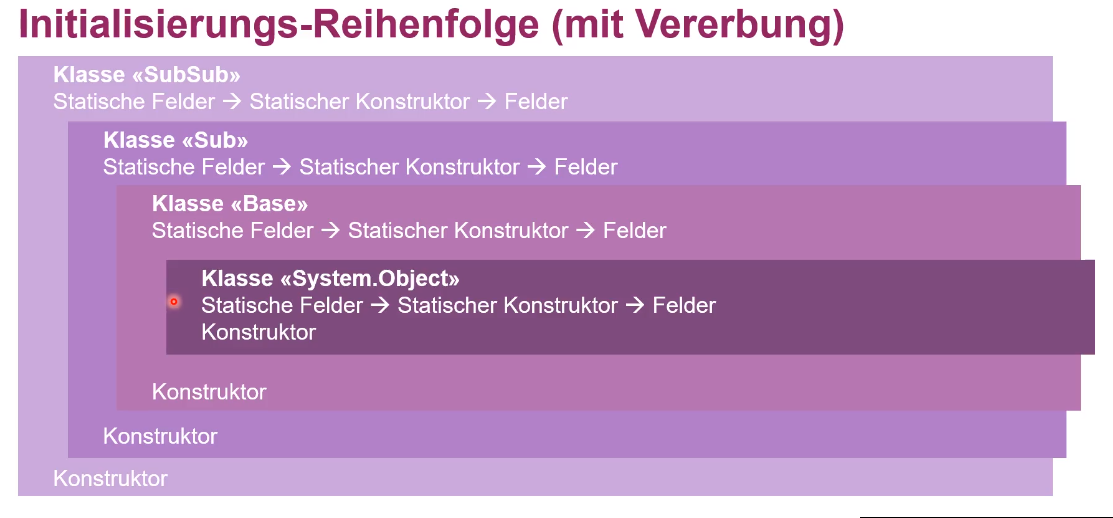
\includegraphics[width=.9\linewidth]{img/initialisierungsreihenfolge.png}
\label{orgc1b0492}
\end{center}

\textbf{Type Casting}

\texttt{null} could be also casted.
Except you want to cast it in a Value Type (\href{../../../roam/20211008085202-struct_in_c.org}{Struct in C\#}).
This would throw an \texttt{InvalidCastException}.
\lstset{language=csharp,label= ,caption= ,captionpos=b,numbers=none}
\begin{lstlisting}
SubSub a = new SubSub();
if (a is SubSub) {}
\end{lstlisting}

\texttt{obj as T} short for \texttt{obj is T ? (T)obj : (T)null}
\lstset{language=csharp,label= ,caption= ,captionpos=b,numbers=none}
\begin{lstlisting}
Base a = new Sub();
Sub b = a as Sub;

/* Same as following*/
Sub b = a is Sub ? (Sub)a : (Sub)null;
\end{lstlisting}

\lstset{language=csharp,label= ,caption= ,captionpos=b,numbers=none}
\begin{lstlisting}
Base a = new SubSub();
if (a is SubSub casted) {
    Console.WriteLine(casted);
}

/* same as following*/ 
SubSub casted = default;
if (a is SubSub) {
    casted = (SubSub) a;
}
\end{lstlisting}

\textbf{Override Functions}

So that you can override a function it has to be marked as \texttt{virtual} in the base class.
In the child class you can override it with the keyword \texttt{override}.
The keyword \texttt{virtual} is not possible when:
\begin{itemize}
\item function is static
\item function is \texttt{abstract} (implied virtual)
\item private (not even possible to override)
\item override (implied virtual from base class)
\end{itemize}


\textbf{Dynamic Binding in C\#}

Rule Set in pseudo code:
\lstset{language=csharp,label= ,caption= ,captionpos=b,numbers=none}
\begin{lstlisting}
var st = static type of obj;
var dt = dynamic type of obj;
var m = Method "M" of st; // Standard-Methode, existiert zwingend (evtl. vererbt)!
var typelist = all types between st (exclusive) and dt (inclusive);

foreach (var t in typelist)
{
    // Schlüsselwort "override"
    if (t has an override method "M")
	m = Method "M" of t;
    // Schlüsselwort "new"
    // Oder ohne Angabe
    else if (t has a non-override method "M")
	break;
}
call m;
\end{lstlisting}

\textbf{Interrupt dynamic binding}

If the keyword \texttt{override} is missing the original functions are hidden therefore the dynamic binding is interrupted.
If you want this you should add the \texttt{new} keyword: \texttt{public new void I() \{\}}.
This tells the compiler that you really want this and it is not a mistake.

\textbf{seald keyword}

With the keyword \texttt{sealed} you prevent that something inherits from this.
\texttt{sealed} can be used with classes, properties, indexers and events.

\texttt{sealed} can improve the performance because the dynamic binding algorithm is not executed.

sealed members are not very common and are only possible with the keyword \texttt{override}:
\begin{itemize}
\item \texttt{public override sealed void Add()}
\end{itemize}


But you can hide the sealed function and create a new hierarchy with the \texttt{new} keyword:
\begin{itemize}
\item \texttt{public new virtual void Add()}
\end{itemize}


\textbf{Interfaces in C\#}

Because \href{../../../roam/20211003114158-c.org}{C\#} does not allow multiple inheritance the Interfaces are created.
A class can implemented multiple interfaces at the same time.
All function defined in the interface must be implemented by the class or by a base class.
Implementation of Interface members must be \texttt{public} and must not be \texttt{static}.
Interfaces can inherit from other Interfaces

\textbf{Naming Clashes using Interfaces}

If your class implements two interfaces with the same name and same signature you have 3 possible solutions:
\begin{enumerate}
\item implement the method regularly.
The implementation counts for both interfaces
\begin{itemize}
\item do this if the logic for both interfaces are the same
\end{itemize}
\item implement the methods explicit
\begin{itemize}
\item do this if the logic for both interfaces are different
\item \texttt{void ISequence.Add(object x) \{ /* do something */ \}}
\item \texttt{void IShoppingCart.Add(object x) \{ /* do something */ \}}
\end{itemize}
\item implement one regularly and one explicit
\begin{itemize}
\item this is useful if the regularly one should be the default
\end{itemize}
\end{enumerate}

\lstset{language=csharp,label= ,caption= ,captionpos=b,numbers=none}
\begin{lstlisting}
class ShoppingCart : ISequence, IShoppingCart {
    void ISequence.Add(object x) {}
    void IShoppingCart.Add(object x) {}
}

ISequence sc1 = new ShoppingCart();
sc1.Add("Hello");

IShoppingCart sc2 = new ShoppingCart();
sc2.Add("Hello");
\end{lstlisting}

\lstset{language=csharp,label= ,caption= ,captionpos=b,numbers=none}
\begin{lstlisting}
class ShoppingCart : ISequence, IShoppingCart {
    void Add(object x) {} // will be the default
    void IShoppingCart.Add(object x) {}
}
\end{lstlisting}

\textbf{Delegates}

Delegates are type safe function pointers as a object (reference type).
Internally it holds references to 0 to n methods.

\lstset{language=csharp,label= ,caption= ,captionpos=b,numbers=none}
\begin{lstlisting}
public delegate void Notifier(string sender);
public static void SayHi(string sender);


Notifier greetings;
greetings = new Notifier(SayHi);
// kurzform
greetings = SayHi;
greetings("John");
\end{lstlisting}

\emph{Attention}: Delegates must not be \texttt{null} if you want to invoke it.
\lstset{language=csharp,label= ,caption= ,captionpos=b,numbers=none}
\begin{lstlisting}
if (delegateVar != null) {
    delegateVar(params);
}

// neu ab C# 6.0
delegateVar?.Invoke(params);
\end{lstlisting}

\lstset{language=csharp,label= ,caption= ,captionpos=b,numbers=none}
\begin{lstlisting}
// Anonymous delegate
delegate bool Predicate(string s);
private static void DoSomething(Predicate pred) { /**/ }

DoSomething(delegate(string s){
	return s.StartsWith('S');
    });
\end{lstlisting}


\textbf{Multicast Delegates}

Technical all delegates are multicast delegates. Normal delegates are just a special case where the delegates hold only one reference to a function.

Delegates are taken by the compiler and generates from it a new class which inherits from the class \texttt{MulticastDelegate}. Only the compiler can use the \texttt{MulticastDelegate} class.

The compiler also generates from this \texttt{greetings("John");} the following snippet:
\lstset{language=csharp,label= ,caption= ,captionpos=b,numbers=none}
\begin{lstlisting}
foreach(Delegate dele in greetings.GetInvocationList()) {
    ((Notifier)dele).Invoke("John")
}
\end{lstlisting}

\emph{Attention}: Do not use return values, out or ref parameters in Multicast Delegates.
Only the values form the last function call are returned. 


\textbf{Manipularting Multicast Delegates}

To manipulate the delegate three operations exits:
\begin{itemize}
\item \texttt{=} assigns a function to the delegate
\item \texttt{+=} adds a function to the delegate
\item \texttt{-=} removes a function from the delegate
\end{itemize}


Functions are executed in the same order as you added (\texttt{+=}) it to the Multicast Delegate.
The newest function witch matches is removed when using \texttt{-=}.

\textbf{Implementation Multicast Delegate}

A delegate is implemented as a \href{../../../roam/20210806213600-linkedlist.org}{LinkedList} and stores three things:
\begin{itemize}
\item target: reference to the target object
\begin{itemize}
\item the instance of the class, if static \texttt{null}
\end{itemize}
\item method: the method reference
\item perv: the reference to the previous delegate
\end{itemize}


\begin{center}
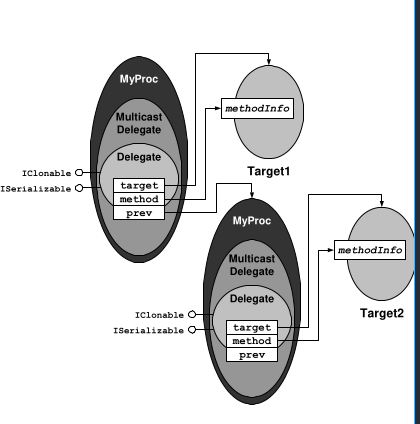
\includegraphics[width=.9\linewidth]{img/multicast_delegate_implementation.png}
\label{org4a38fbb}
\end{center}


\textbf{Predefined Generic Delegates}
\emph{Action}:
\begin{itemize}
\item \texttt{Action()}
\item \texttt{Action<in T>(T obj);}
\item \texttt{Action<in T1, ..., in T16>(T obj, ..., T16 arg);}
\end{itemize}

\emph{Func}:
\begin{itemize}
\item \texttt{TResult Func<out TResult>()}
\item \texttt{TResult Func<in T, out TResult>(T arg)}
\item \texttt{TResult Func<in T, ..., in T16, out TResult>(T arg, ..., T16 arg16)}
\item The last type parameter is the result type
\end{itemize}

\emph{Predicate}:
\texttt{delegate bool Predicate<in T>(T obj);}

\emph{EventHandler}:
\begin{itemize}
\item \texttt{EventHandler<TEventArgs>(object sender, TEventArgs e);}
\item \texttt{EventHandler(object sender, EventArgs e);}
\end{itemize}


\textbf{Events}

Events are just syntactical sugar.
The compiler takes the event and generates a private delegate and adds (un)subscribe logic as public (\texttt{+=} and \texttt{-=}).
\lstset{language=csharp,label= ,caption= ,captionpos=b,numbers=none}
\begin{lstlisting}
public delegate void TickEventHandler(int ticks, int interval);

public class Clock {
    public event TickEventHandler OnTickEvent;

    /* event is transformed to */
    private TickEventHandler OnTickEvent;
    public void add_OnTickEvent(TickEventHandler h) { OnTickEvent += h; }
    public void remove_OnTickEvent(TickEventHandler h) { OnTickEvent -= h; }
}
\end{lstlisting}


The default syntax of the events is the following:
\lstset{language=csharp,label= ,caption= ,captionpos=b,numbers=none}
\begin{lstlisting}
public delegate void AnyHandler(object sender, AnyEventArgs e);
\end{lstlisting}

\begin{itemize}
\item \texttt{object sender}: the sender of the event, the sender hands \texttt{this} over at the call of the delegate / event
\item \texttt{AnyEventArgs e}: an arbitrary sub class ob \texttt{EventArgs}. It contains information to the event.
\end{itemize}


\textbf{Anonymous Methods}

In \href{../../../roam/20211003114158-c.org}{C\#} you can create anonymous methods with delegates or with lambdas.
Anonymous methods can not use \texttt{params[]}, \texttt{ref} and not \texttt{out} parameters.

\emph{Delegates}:
\lstset{language=csharp,label= ,caption= ,captionpos=b,numbers=none}
\begin{lstlisting}
list.ForEach(delegate(int i) { Console.WriteLine(i); });

int sum = 0;
list.ForEach(delegate(int i) { sum += i; });
list.ForEach(delegate(int i) { sum += 1; });
\end{lstlisting}

\emph{Lambda}:
\lstset{language=csharp,label= ,caption= ,captionpos=b,numbers=none}
\begin{lstlisting}
List<int> list = new List<int>();
int sum = 0;
list.ForEach(element => sum += element);
\end{lstlisting}

\begin{center}
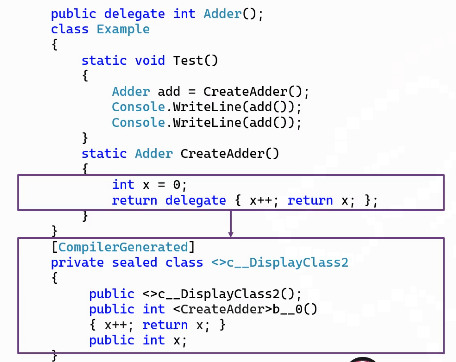
\includegraphics[width=.9\linewidth]{img/closures_how_does_it_work.png}
\label{orgb86455a}
\end{center}

\section{Generic / Nullable}
\label{sec:orge116722}

\textbf{Benefits}
When you use generics in a .NET project you got the following benefits:
\begin{itemize}
\item reusability
\item type safety
\item performance improvements
\end{itemize}


The performance improvements is only available for value types.
The improvement is obtained by the fact that this types does not need to be boxed / unboxed.
With \texttt{object} you would always have to do a boxing / unboxing.

\textbf{Types of Constraints}

For the generic type T you have 6 possible constraints:
\begin{itemize}
\item struct - T must be a struct
\item class - T must be a class
\item new() - T must have a default constructor
\item ClassName - T must inherit from ClassName
\item InterfaceName - T must implement InterfaceName
\item TBase - T must be equal to TBase or T has to inherit from TBase
\end{itemize}


\lstset{language=csharp,label= ,caption= ,captionpos=b,numbers=none}
\begin{lstlisting}
class Something<T, K>
    where T : struct, class, new()
    where K : ISequence
{
    /* fields, methods, properties, ...*/
}
\end{lstlisting}

\textbf{Generic Type Inference}

If the type parameters is redundant it can be omitted.
This is the case if \texttt{T} is formal parameter.
If \texttt{T} is only the return value or not in the signature the type has to be written.
\lstset{language=csharp,label= ,caption= ,captionpos=b,numbers=none}
\begin{lstlisting}
public void Print<T>(T t) { /**/ }
public T Get<T>() { /**/ }

Print<int>(12);
Print(12);

int i1 = Get<int>();
int i2 = Get(); // Compiler error
\end{lstlisting}

\textbf{How do Generics Work}

The value types are treated different than the reference types.
When the runtime sees the first occurrence of a struct as a generic it generates a new concrete class where \texttt{T} is replaced with the struct.
By value types during the runtime the \texttt{T=is replaced with =object} (same as in \href{../../../roam/20201116150053-java.org}{Java}).


\textbf{Whate are Nullable Values}

Nullable value type is a normal struct which is implemented as following:
\lstset{language=csharp,label= ,caption= ,captionpos=b,numbers=none}
\begin{lstlisting}
public struct Nullable<T>
    where T : struct {
	public Nullable(T value);
	public bool HasValue { get; }
	public T Value { get; }
    }
\end{lstlisting}

The compiler adds some syntactical sugar for easier usage:
\lstset{language=csharp,label= ,caption= ,captionpos=b,numbers=none}
\begin{lstlisting}
int? x = 123;
Nullable<int> x = 123;
int? x = null;
\end{lstlisting}

For secure reading the following methods should be used:
\begin{itemize}
\item \texttt{GetValueOrDefault()}
\item \texttt{GetValueOrDefault(<default>)}
\end{itemize}


\textbf{Nullable Type Operators}
\lstset{language=csharp,label= ,caption= ,captionpos=b,numbers=none}
\begin{lstlisting}
int i = GetNullableInt() ?? -1;

/* same as */
int? iTemp = GetNullableInt();
int i;
if (!iTemp.HasValue) { i = -1; }
else { i = iTemp.GetValueOrDefault(); }
\end{lstlisting}

\lstset{language=csharp,label= ,caption= ,captionpos=b,numbers=none}
\begin{lstlisting}
int? i = null;
i ??= 1234;

/* same as*/
int? i = null;
i = i ?? 1234;

int? i = null;
int iTemp = i.GetValueOrDefault();
if (!i.HasValue) { iTemp = 1234; }
i = iTemp;

\end{lstlisting}


The \texttt{?.} (Null-conditional operator) is used for secure method chaining:
\lstset{language=csharp,label= ,caption= ,captionpos=b,numbers=none}
\begin{lstlisting}
string s = GetNullableInt()?.ToString();
\end{lstlisting}
Often also used with delegates \href{../../../roam/20211029145415-delegates_in_c.org}{Delegates in C\#}: \texttt{a?.Invoke()}

\section{Exception}
\label{sec:orgf467813}

\textbf{Exceptions}

All Exceptions in \href{../../../roam/20211003114158-c.org}{C\#} inhert from \texttt{System.Exception} and are unchecked exceptions (diffrent in \href{../../../roam/20201116150053-java.org}{Java}).

In \href{../../../roam/20211003114158-c.org}{C\#} you throw an exception with the \texttt{throw} keyword.
\lstset{language=csharp,label= ,caption= ,captionpos=b,numbers=none}
\begin{lstlisting}
throw new Exception("Failure");
\end{lstlisting}

\textbf{Rethrow Exception}

In \href{../../../roam/20211003114158-c.org}{C\#} you can throw an exception in two ways:
\begin{enumerate}
\item Cut the Stack Trace
\item Continue the Stack Trace
\end{enumerate}

Cut the Stack Trace:
\lstset{language=csharp,label= ,caption= ,captionpos=b,numbers=none}
\begin{lstlisting}
try {
    throw new Exception("Failure");
}
catch (Exception e) {
    throw e;
}
\end{lstlisting}

Continue the Stack Trace (also called \emph{rethrowing}).
\lstset{language=csharp,label= ,caption= ,captionpos=b,numbers=none}
\begin{lstlisting}
try{
    throw new Exception("Failure");
}
catch (Exception e) {
    throw;
}
\end{lstlisting}

\textbf{Exception Handling with Multicast Delegates}

If in a function inside of a Multicast Delegate an exception occurs, the following functions (F2 in \ref{org21d3e8e}) are not executed.
Even if in the caller method a try-catch block exists.

\begin{center}
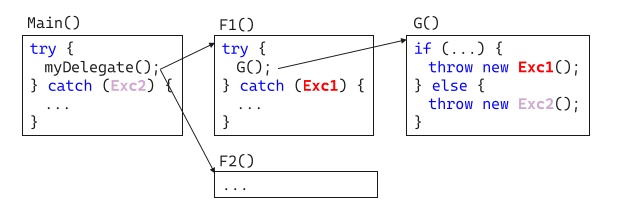
\includegraphics[width=.9\linewidth]{img/exception_with_multicast.png}
\label{org21d3e8e}
\end{center}

\textbf{Exception Filters}

In some cases you want that an exception is only catch if a specific condition is fulfilled.
This can be achieved with Exception Filters.

\lstset{language=csharp,label= ,caption= ,captionpos=b,numbers=none}
\begin{lstlisting}
try
{
    /* ... */
}
catch (Exception e) when (DateTime.Now.Hour < 18)
{
    /* ... */
}
catch (Exception e) when (DateTime.Now.Hour >= 18)
{
    /* ... */
}
\end{lstlisting}

\textbf{Check Arguments}

For checking the arguments in \href{../../../roam/20211003114158-c.org}{C\#} you have the \texttt{ArgumentNullException} and the \texttt{ArgumentOutOfRangeExceptioArgumentOutOfRangeException}.
Use always the \texttt{nameof} operator in this case because it is refactoring stable (Not just a hard coded string you give as a parameter to the constructor).

\lstset{language=csharp,label= ,caption= ,captionpos=b,numbers=none}
\begin{lstlisting}
string Replicate(string s, int nTimes)
{
    if (s == null)
    {
	throw new ArgumentNullException(
	    nameof(s));
    }
    if (s.Length == 0)
    {
	throw new ArgumentOutOfRangeException(
	    nameof(s));
    }
    if (nTimes <= 1)
    {
	throw new ArgumentOutOfRangeException(
	    nameof(nTimes));
    }
    return new StringBuilder()
	.Insert(0, s, nTimes)
	.ToString();
}
\end{lstlisting}

\section{Foreach / Iterator / Extension Methods}
\label{sec:orgf2ab320}

\textbf{foreach}

While an iterator is active on a collection, it is \textbf{not} possible to modify this collection.

\textbf{foreach compiled output}

The compiler converts the following foreach loop in a while loop.

\lstset{language=csharp,label= ,caption= ,captionpos=b,numbers=none}
\begin{lstlisting}
foreach (int i in list)
{
    if (i == 3) continue;
    if (i == 5) break;
    Console.WriteLine(i);
}
\end{lstlisting}

\lstset{language=csharp,label= ,caption= ,captionpos=b,numbers=none}
\begin{lstlisting}
// Compiler Output
IEnumerator enumerator = list.GetEnumerator();
try
{
    while (enumerator.MoveNext())
    {
	int i = (int)enumerator.Current;
	if (i == 3) continue;
	if (i == 5) break;
	Console.WriteLine(i);
    }
}
finally
{
    IDisposable disposable
	= enumerator as IDisposable;
    if (disposable != null)
	disposable.Dispose();
}
\end{lstlisting}

\textbf{Make Collection foreach-able}

If you want to use your collection in a foreach loop your collection must implemented the \texttt{IEnumerable} / \texttt{IEnumerable<T>} interface or functions with the same signature and name. 

\textbf{yield keyword}

The \texttt{yield} keyword is used to create deferred evaluated functions.
It exits two versions of \texttt{yield}:
\begin{itemize}
\item \texttt{yield return}: returns the next value
\item \texttt{yield break}: terminated the iteration
\end{itemize}


The \texttt{yield} keyword tells the compiler that it should generate a state machine.
After each call of the method a other (the next) element is returned until know elements are remaining in the colleciton.

\textbf{Iterator Methods}

Iterator methods have always the same signature and min. one \texttt{yield} keyword:
\begin{itemize}
\item \texttt{public IEnumerator <Name>()}
\item \texttt{public IEnumerator<T> <Name>()}
\end{itemize}


A iterator method returns always an \href{../../../roam/20211118154822-iterator.org}{Iterator}.
The call of \texttt{GetEnumerator} does not execute the function.
Only the call of \texttt{MoveNext()} on the iterator.
This is called Deffered Evaluation.

The default iterator method is \texttt{GetEnumertor} but you can create custom functions or properties:
\lstset{language=csharp,label= ,caption= ,captionpos=b,numbers=none}
\begin{lstlisting}
public IEnumerator<int> GetEnumerator() {
    for (int i = 0; i < data.Length; i++)
	yield return data[i];
}
// Spezifische Iterator-Methode
public IEnumerable<int> Range(int from, int to) {
    for (int i = from; i < to; i++)
	yield return data[i];
}
// Spezifisches Iterator-Property
public IEnumerable<int> Reverse {
    get {
	for (int i = data.Length - 1; i >= 0; i--)
	    yield return data[i];
    }
}
\end{lstlisting}


This methods can be used inside a foreach loop.
\lstset{language=csharp,label= ,caption= ,captionpos=b,numbers=none}
\begin{lstlisting}
foreach (int elem in list.Range(2, 7)) { /**/ }
\end{lstlisting}

\textbf{Extension Method}

Extension Methods are a compiler feature of \href{../../../roam/20211003114158-c.org}{C\#} which allows you to extend a class from the user view.
In reality the class is not extend.
It is \emph{not} possible to access private members of the extended class.
If a conflict occurrs always the method from the class itself is used.

\textbf{How to create extension Methods}

Extension Methods have the following requirements:
\begin{itemize}
\item must be inside a static class
\item the function itself must be static
\item the first parameter must be \texttt{this}
\begin{itemize}
\item this describes on which classes the function can be executed on
\end{itemize}
\end{itemize}

\lstset{language=csharp,label= ,caption= ,captionpos=b,numbers=none}
\begin{lstlisting}
public static class ExtensionMethods
{
    static string ToStringSafe(this object obj)
    {
	return obj == null ? string.Empty : obj.ToString();
    }

    public static void Test()
    {
	1.ToStringSafe();
	/* turns into */
	ExtensionMethods.ToStringSafe(1);
    }
}
\end{lstlisting}

\section{Lambda / Query Expression}
\label{sec:org01d4ba5}

\textbf{Lambda Expression}

In \href{../../../roam/20211003114158-c.org}{C\#} exits two kind of Lambdas:
\begin{itemize}
\item \emph{Expression Lambdas}:  \texttt{(<parameters>) => expression}
\item \emph{Statement Lambdas}: \texttt{(<parameters>) => \{ staments; \}}
\end{itemize}


Lambdas should not be longer than 2 - 3 statements.
If you need more statements is worthy to think about to write a complete function.

\textbf{Expression-Bodied Members}

Expression-Bodied Members are a special kind of Lambdas.
This lambdas contain only one statement can be used instead of the \texttt{\{\}} block.

\textbf{Object / Collection Initializers}

Sometimes you have to create a object hierarchy.
Normally you have to create each object first and then set the properties.
Using the Object / Collection Initializers it is possible to write this in one step.
Then the compiler generate from your code what you normally have to do by your self.

\lstset{language=csharp,label= ,caption= ,captionpos=b,numbers=none}
\begin{lstlisting}
Student s1 = new Student();
s1.Name = "Hans Muster";
s1.Id = 1;

Student s2 = new Student();
s2.Name = "Joe Doe";
s2.Id = 2;

Course c = new Course();
c.Name = "MsTe";
c.Students = new List();
c.Students.Add(s1);
c.Students.Add(s2);
\end{lstlisting}

\emph{Object / Collection Initializers}
\lstset{language=csharp,label= ,caption= ,captionpos=b,numbers=none}
\begin{lstlisting}
Course c = new Course {
    Name = "MsTe",
    Students = new List {
	new Student {
	    Name = "Hans Muster",
	    Id = 1
	},
	new Student {
	    Name = "Joe Doe",
	    Id = 2
	},
    }
};
\end{lstlisting}

\textbf{Anonymous Types}

Anonymous Types are used to store an intermediate result.
This is often used in LINQ queries.
To use anonymous types you must use the \texttt{var} keyword.
All properties are \texttt{readonly}.
The functions \texttt{Equals()}, \texttt{GetHashCode()} and \texttt{ToString()} are overwritten.

\lstset{language=csharp,label= ,caption= ,captionpos=b,numbers=none}
\begin{lstlisting}
var a = new { Id = 1, Name = "John" };
var b = new { a.Id, a.Name };
var studentList = new List<Student>();
var q = studentList
    .GroupBy(s => s.Subject)
    .Select(
	grp => new {
	    Subject = grp.Key,
	    Count = grp.Count() });
\end{lstlisting}

The compiler detects that \texttt{a} and \texttt{b} are from the same type. 

\section{LINQ}
\label{sec:org86b237a}
\textbf{What is LINQ}

\emph{LINQ} is short for \emph{Language Integrated Query} and is a compiler feature which uses Extensions Methods extensively.
Most Query Operators are implemented als deffered functions.
A few are implemented as immediate.
This are normally function which do not return an \texttt{IEnumerable} like \texttt{ToList} or \texttt{Count}.


\lstset{language=csharp,label= ,caption= ,captionpos=b,numbers=none}
\begin{lstlisting}
string[] cities = { "Bern", "Basel" };

var q1 = from c in cities select c;
/* is turn into */
var l1 = cities.Select(c => c);

var q2 = from c in cities where c.StartsWith("B") orderby c select c;
/* is turn into */
var l2 = cities.Where(c => c.StartsWith("B")).OrderBy(c => c);
\end{lstlisting}

\textbf{LINQ Query Syntax}

The Syntax components from LINQ.


\begin{center}
\begin{tabular}{ll}
keyword & description\\
\hline
from & defines range variable and data source\\
where & filter\\
orderby & sort\\
select & projection on a element type\\
group & group into a sequence of group elements\\
join & link two data sources\\
let & define a support variable\\
\end{tabular}
\end{center}


\lstset{language=csharp,label= ,caption= ,captionpos=b,numbers=none}
\begin{lstlisting}
var q1 = from s in Students
    where s.Subject == "Computing"
    orderby s.Name
    select new {s.Id, s.Name };
\end{lstlisting}

\textbf{Group with LINQ}

\lstset{language=csharp,label= ,caption= ,captionpos=b,numbers=none}
\begin{lstlisting}
var q = from s in Students
    group s.name by s.Subject;

foreach (var group in q)
{
    Console.WriteLine(group.Key);
    foreach (var name in group)
    {
	Console.WriteLine(" " + name);
    }
}
\end{lstlisting}

\begin{verbatim}
Computing
  John
  Sue
Mathematics
  Ann
  Bob
\end{verbatim}

\textbf{Group Into with LINQ}

\lstset{language=csharp,label= ,caption= ,captionpos=b,numbers=none}
\begin{lstlisting}
var q = from s in Students
    group s.name by s.Subject into g
    select new
    {
	Field = g.Key(),
	N = g.Count()
    };

foreach (var x in q)
{
    Console.WriteLine(x.Field + ":" + x.N);
}
\end{lstlisting}
\begin{verbatim}
Computing: 2
Mathematics: 2
\end{verbatim}

\textbf{Inner Join with LINQ}

\emph{Explizit}:
\lstset{language=csharp,label= ,caption= ,captionpos=b,numbers=none}
\begin{lstlisting}
var q = from s in Students
    join m in Markings
    on s.Id equals m.StudentId
    select s.Name + ", " + m.Course + ", " + m.Mark;
\end{lstlisting}

\emph{Implizit}: (builds Cross product and filter it with \texttt{where}) - do not use it when possible (slow)
\lstset{language=csharp,label= ,caption= ,captionpos=b,numbers=none}
\begin{lstlisting}
var q =
    from s in Students
    from m in Markings
    where s.Id == m.StudentId
    select s.Name + ", " + m.Course + ", " + m.Mark;
\end{lstlisting}
\begin{verbatim}
John Doe, Programming, 3
John Doe, Database, 2
Linda Miller: Organic Chemistry, 1
\end{verbatim}

\textbf{Group Joins with LINQ}

LINQ groups by the part in the \texttt{from} part (\texttt{s} in the example).
Therefore, everything which belongs \texttt{s} is put in a list (\texttt{into list}).

In this example for each student a list is created with all markings belonging to it.
\lstset{language=csharp,label= ,caption= ,captionpos=b,numbers=none}
\begin{lstlisting}
var q =
    from s in Students
    join m in Markings
    on s.Id equals m.StudentId
    into list
    select new
    {
	Name = s.Name,
	Marks = list
    };

foreach (var group in q)
{
    Console.WriteLine(group.Name);
    foreach(var m in group.Marks)
    {
	Console.WriteLine(m.Course);
    }
}
\end{lstlisting}

\textbf{Left Outer Joins with LINQ}

\lstset{language=csharp,label= ,caption= ,captionpos=b,numbers=none}
\begin{lstlisting}
var q = from s in Students
    join m in Markings
    on s.Id equals m.StudentId
    into list
    from sm in list.DefaultIfEmpty()
    select s.Name + ", " + (sm == null ? "?" : sm.Course + ", " + sm.Mark);

foreach (var x in q)
{
    Console.WriteLine(x);
}
\end{lstlisting}
\begin{verbatim}
John Doe, Programming, 3
John Doe, Database, 2
Linda Miller, Organic Chemistry, 1
Ann Forster, ?
\end{verbatim}

\textbf{Let with LINQ}

\texttt{let} allows to create support variables.

\lstset{language=csharp,label= ,caption= ,captionpos=b,numbers=none}
\begin{lstlisting}
var result =
    from s in Students
    let year = s.Id / 1000
    where year == 2009
    select s.Name + " " + year.ToString();

foreach (string s in result)
{
    Console.WriteLine(s);
}
\end{lstlisting}

\begin{verbatim}
John Doe 2009
Linda Miller 2009
\end{verbatim}

\textbf{SelectMany with LINQ}

Allows you zu summarize a nested list into one list.

\lstset{language=csharp,label= ,caption= ,captionpos=b,numbers=none}
\begin{lstlisting}
var list = new List<List<string>>
{
    new List<string> { "a", "b", "c" },
    new List<string> { "1", "2", "3" },
    new List<string> { "ö", "ä", "ü" },
};

var q1 = list.SelectMany(s => s);
// q2 same as q1
var q2 = from segment in list
    from token in segment
    select token;


foreach (string lie in q1)
{
    Console.WriteLine("{0}.", line);
}
\end{lstlisting}
\begin{verbatim}
a.b.c.1.2.3.ö.ä.ü
\end{verbatim}

\section{Async}
\label{sec:orgdaf7922}
\textbf{Task in .NET}

Task are a lightweight variant of a Thread and are normally used in \texttt{async} / \texttt{await} cases.

\textbf{Task vs. Thread}

A Task has a return value and can run multiple operations in parallel.
A Thread has no return value and has only one operation.
In general a Task is a more \emph{high level} construct and easier to use.
But with a Thread you have more control over the details.

\textbf{async vs. parallel}

\emph{Attention:} Asynchron (Concurrent) ist not the same as parallel (see \ref{org8e38660}).

\begin{center}
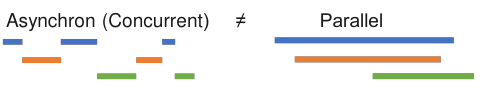
\includegraphics[width=.9\linewidth]{img/async_vs_concurrent.png}
\label{org8e38660}
\end{center}

\textbf{Async / Await operations}

To avoid the problems of a blocking task you can wait on the task asynchronously.
This can be achieved over callbacks or the functions returns a task object.
Normally you can / should implement IO operations as async.

\textbf{Blocking Task}

\emph{Attention:} synchronous waits on a task are most of the time not desired because they block the current Thread.
If it's the UI Thread then the UI is not responding and it looks like the application is not working anymore.


Blocking API:
\begin{itemize}
\item \texttt{Task.Result}
\item \texttt{Task.Wait()}
\item \texttt{Task.WaitAll()}
\end{itemize}


\textbf{async in .NET}

A async function in \href{../../../roam/20211003114703-net.org}{.NET} can only have the following return types:
\begin{itemize}
\item \texttt{Task}
\item \texttt{Task<T>}
\item \texttt{void} (fire and forget, should only be used in exceptional cases)
\end{itemize}


\textbf{await in .NET}

The \texttt{await} keyword waits on the Task to fulfill.
If the task is fulfilled then the execution is continued.
An alternative for await are continuations and basically the same.

\lstset{language=csharp,label= ,caption= ,captionpos=b,numbers=none}
\begin{lstlisting}
// await syntax
int id = await GetSomeCustomerId();
string t2 = await GetOrders(id);
Console.WriteLine(t2);

// continuations
Task<int> t1 = GetSomeCustomerId();
t1.ContinueWith(id =>
{
    Task<string> t2 = GetOrders(id.Result);
    t2.ConinueWith(order =>
		   Console.WriteLine(order.Result)
    );
});
\end{lstlisting}

\section{Reflection}
\label{sec:org85482dd}
\textbf{Usage of reflection}

The most prominent application for reflection is \emph{Intelli Sense} or the \emph{Object Browser} in Visual Studio.
Using reflection you can do the following:
\begin{itemize}
\item Type Discovery
\item Late Binding (Method / Properties)
\item Reflection Emit / Code-Emittierung
\end{itemize}


\textbf{System.Type}

All types in the \href{../../../roam/20211003114644-common_language_runtime.org}{CLR} are self defined using \texttt{System.Type}.
The \texttt{System.Type} is the entry point for all reflection operations.
The \texttt{System.Type} class describes itself with an \texttt{System.Type} instance.
The base class for \texttt{System.Type} is the \texttt{System.RuntimeType}.

\textbf{Runtime Prefix}

The prefix \emph{Runtime} in .NET means that this class is only instanced only once.
For example the \texttt{System.RuntimeType}.

\textbf{Get a System.Type}

For every type a \texttt{System.Type} can be obtained with \texttt{typeof} or \texttt{GetType()}.

\lstset{language=csharp,label= ,caption= ,captionpos=b,numbers=none}
\begin{lstlisting}
int someInt = 2;
var type = someInt.GetType();
var type2 = typeof(int);
\end{lstlisting}


\begin{center}
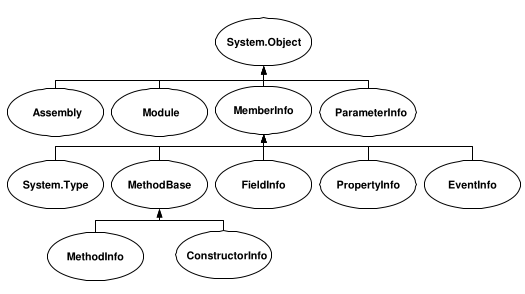
\includegraphics[width=.9\linewidth]{img/type_hierarchy_reflection.png}
\label{org2b5d679}
\end{center}

\textbf{Type discovery}

\lstset{language=csharp,label= ,caption= ,captionpos=b,numbers=none}
\begin{lstlisting}
Assembly a01 = Assembly.Load("mscorlib");
Type[] t01 = a01.GetTypes();
foreach (Type type in t01)
{
    Console.WriteLine(type);
    MemberInfo[] mInfos = type.GetMembers();
    foreach (var mi in mInfos)
    {
	Console.WriteLine(
	    "\t{0}\t{1}",
	    mi.MemberType,
	    mi);
    }
}
\end{lstlisting}

\begin{verbatim}
System.Int32
  Method Int32 CompareTo(System.Object)
  Method Int32 CompareTo(Int32)
  Method Boolean Equals(System.Object)
  Method Boolean Equals(Int32)
  Method Int32 GetHashCode()
  Method System.String ToString()
\end{verbatim}

\textbf{Read members}

\emph{All members}
\lstset{language=csharp,label= ,caption= ,captionpos=b,numbers=none}
\begin{lstlisting}
Type type = typeof(Counter);
MemberInfo[] miAll = type.GetMembers();
foreach (MemberInfo mi in miAll)
{
    Console.WriteLine("{0} is a {1}",
		      mi, mi.MemberType);
}
Console.WriteLine("----------");
PropertyInfo[] piAll = type.GetProperties();
foreach (PropertyInfo pi in piAll)
{
    Console.WriteLine("{0} is a {1}",
		      pi, pi.PropertyType);
}
\end{lstlisting}

\begin{verbatim}
Int32 get_CountValue() is a Method
Void set_CountValue(Int32) is a Method
Void Increment() is a Method
Void Decrement() is a Method
String ToString() is a Method
Boolean Equals(Object) is a Method
Int32 GetHashCode() is a Method
Type GetType() is a Method
Void .ctor(Int32) is a Constructor
Int32 CountValue is a Property
PropertyChangedEventHandler PropertyChanged
  is a Event
----------
Int32 CountValue is a Property
\end{verbatim}

\emph{Dynamically}
\lstset{language=csharp,label= ,caption= ,captionpos=b,numbers=none}
\begin{lstlisting}
Type type = typeof(Assembly);
BindingFlags bf =
    BindingFlags.Public |
    BindingFlags.Static |
    BindingFlags.NonPublic |
    BindingFlags.Instance |
    BindingFlags.DeclaredOnly;

MemberInfo[] miFound =
    type.FindMembers(
	MemberTypes.Method,
	bf,
	Type.FilterName,
	"Get*"
    );
\end{lstlisting}

\textbf{Field info}

The field info class describes a single field of a class.
This includes:
\begin{itemize}
\item Name
\item Type
\item Visibility
\item and more
\end{itemize}


It allows you to read and write regardless the visibility of the field:
\begin{itemize}
\item \texttt{object GetValue(object obj);}
\item \texttt{void SetValue(object obj, object value)}
\end{itemize}


But try to prevent to set values over this way.
Especially if the field is private / protected.


\lstset{language=csharp,label= ,caption= ,captionpos=b,numbers=none}
\begin{lstlisting}
Type type = typeof (Counter);
Counter c = new Counter(1);
// All Fields
FieldInfo[] fiAll = type.GetFields(
    BindingFlags.Instance |
    BindingFlags.NonPublic);
// Specific Field
FieldInfo fi = type.GetField(
    "countValue",
    BindingFlags.Instance |
    BindingFlags.NonPublic);
int val01 = (int) fi.GetValue(c);
c.Increment();
int val02 = (int) fi.GetValue(c);
fi.SetValue(c, -999);
\end{lstlisting}

\textbf{Property Info}

The property info describes a property of a class.
This includes the:
\begin{itemize}
\item name
\item type
\item visibility
\item informations to get / set
\end{itemize}


The property info allows you to read / write the property regardless of the visibility:
\begin{itemize}
\item \texttt{object GetValue(object obj);}
\item \texttt{void SetValue(object obj, object value);}
\end{itemize}


But try to prevent to set values over this way when the property is private / protected.


\lstset{language=csharp,label= ,caption= ,captionpos=b,numbers=none}
\begin{lstlisting}
Type type = typeof(Counter);
Counter c = new Counter(1);
// All Properties
PropertyInfo[] piAll = type.GetProperties();
// Specific Property
PropertyInfo pi =
    type.GetProperty("CountValue");
int val01 = (int)pi.GetValue(c);
c.Increment();
int val02 = (int)pi.GetValue(c);
if (pi.CanWrite)
{
    pi.SetValue(c, -999);
}
\end{lstlisting}


\textbf{Method Info}

The method info inherits from \texttt{MethodBase} and describes a method of a class.
This includes the:
\begin{itemize}
\item name
\item parameters / return value
\item visibility
\item and more
\end{itemize}


Using the method \texttt{Invoke()} you can call the method.

\lstset{language=csharp,label= ,caption= ,captionpos=b,numbers=none}
\begin{lstlisting}
/* Without parameters */
Type type = typeof(Counter);
Counter c = new Counter(1);
// All Methods
MethodInfo[] miAll = type.GetMethods();
// Specific Method
MethodInfo mi = type.GetMethod("Increment");
mi.Invoke(c, null);

/* With parameters */
Type type = typeof(System.Math);
Type[] paramTypes = { typeof(int) };
// Get method info for Cos( )
MethodInfo miAbs = type
    .GetMethod("Abs", paramTypes);
// Fill an array with the actual parameters
object[] @params = { -1 };
object returnVal = miAbs.Invoke(type,
				@params);
\end{lstlisting}

\textbf{Constructor Info}

The constructor info inherits from \texttt{MethodBase} and describes a constructor of a class.
This includes:
\begin{itemize}
\item name
\item parameters
\item visibility
\end{itemize}


The constructor can be called using the \texttt{Invoke()} method.

\lstset{language=csharp,label= ,caption= ,captionpos=b,numbers=none}
\begin{lstlisting}
Type type = typeof(Counter);
// All Constructors
ConstructorInfo[] ciAll = type.GetConstructors();
// Specific Constructor Overload 01
ConstructorInfo ci01 = type.GetConstructor(
    new[] { typeof(int) });
Counter c01 = (Counter)ci01.Invoke(
    new object[] { 12 });
// Specific Constructor Overload 02
ConstructorInfo ci02 = type.GetConstructor(
    BindingFlags.Instance|BindingFlags.NonPublic,
    null, new Type[0], null);
Counter c02 = (Counter)ci02.Invoke(null);

/* alternative using activator */
Counter c03 = (Counter)Activator
    .CreateInstance(
	typeof(Counter),
	12 // , "further params", "", ...
    );
// Alternative
// -> when Public Default Constructor exists
Counter c04 = Activator
    .CreateInstance<Counter>();
\end{lstlisting}

\textbf{Attributes in .NET}

Attributes are the same thing like annotations in \href{../../../roam/20201116150053-java.org}{Java}.
They extend the already existing attributes like public, static, abstract or sealed.
All attributes inherit from \texttt{System.Attribute}.

\lstset{language=csharp,label= ,caption= ,captionpos=b,numbers=none}
\begin{lstlisting}
[DataContract, Serializable]
[Obsolete]
// Etc.
    public class Auto
    {
	[DataMember]
	public string Marke { get; set; }
	[DataMember]
	public string Typ { get; set; }
    }
\end{lstlisting}


in \href{../../../roam/20211003114703-net.org}{.NET} exists two kind of attributes:
\begin{itemize}
\item \emph{intrinsic}: in the \href{../../../roam/20211003114644-common_language_runtime.org}{CLR} defined and integrated
\item \emph{custom}: self defined attributes
\end{itemize}


\textbf{Syntax Attribute Usage}

Some attributes can be used multiple times on the same target.

\lstset{language=csharp,label= ,caption= ,captionpos=b,numbers=none}
\begin{lstlisting}
// without parameters
[DataContract]
class a{};

// Named parameters
[DataContract(Name = "AutoClass")]
class b{};

// Positional Paramaters
[Obsolete("Alt!", true)]
class c{};

// mixed
[Obsolete("Alt!", IsError = true)]
class d{};
\end{lstlisting}

\textbf{Create your own attribute}

Your attribute must inherit from \texttt{System.Attribute} and must have the suffix \texttt{Attribute}.
Additionaly it must use the attribute \texttt{AttributeUsage}.
The \texttt{AllowMultiple} is per default set to \texttt{false}.

\lstset{language=csharp,label= ,caption= ,captionpos=b,numbers=none}
\begin{lstlisting}
  [AttributeUsage(
  AttributeTargets.Class |
  AttributeTargets.Constructor |
  AttributeTargets.Field |
  AttributeTargets.Method |
  AttributeTargets.Property,
  AllowMultiple = true)]
      public class BugfixAttribute : Attribute
  {
      public BugfixAttribute(int bugId,
			     string programmer, string date)
      { /* ... */ }
      public int BugId { get; }
      public string Date { get; }
      public string Programmer { get; }
      public string Comment { get; set; }
  }

[Bugfix(121, "Manuel Bauer", "01/03/2015")]
[Bugfix(
107, "Manuel Bauer", "01/04/2015",
Comment = "Some major changes! ;-)")]
    public class MyMath{};
\end{lstlisting}

\textbf{Query an attribute}

\lstset{language=csharp,label= ,caption= ,captionpos=b,numbers=none}
\begin{lstlisting}
Type type = typeof(MyMath);
// All Class Attributes
object[] aiAll =
    type.GetCustomAttributes(true); // true = use also inherited attributes
IEnumerable<Attribute> aiAllTyped =
    type.GetCustomAttributes(
	typeof(BugfixAttribute) /* , true */
    );
// Check Definition
bool aiDef =
    type.IsDefined(typeof(BugfixAttribute));
\end{lstlisting}
\end{multicols}
\end{document}